%% Submissions for peer-review must enable line-numbering
%% using the lineno option in the \documentclass command.
%%
%% Preprints and camera-ready submissions do not need
%% line numbers, and should have this option removed.
%%
%% Please note that the line numbering option requires
%% version 1.1 or newer of the wlpeerj.cls file, and
%% the corresponding author info requires v1.2

\documentclass[fleqn,10pt,lineno]{wlpeerj} % for journal submissions

% ZNK -- Adding headers for pandoc

\setlength{\emergencystretch}{3em}
\providecommand{\tightlist}{
\setlength{\itemsep}{0pt}\setlength{\parskip}{0pt}}
\usepackage{lipsum}
\usepackage[unicode=true]{hyperref}
\usepackage{longtable}



\usepackage{lipsum}

\title{Plant community changes in mountain hay meadows from 2003 to 2017}

\author[1, 2]{Tobias Roth}

\corrauthor[1, 2]{Tobias Roth}{\href{mailto:t.roth@unibas.ch}{\nolinkurl{t.roth@unibas.ch}}}
\author[2]{Lukas Kohli}


\affil[1]{Zoological Institute, University of Basel, Basel, Switzerland}
\affil[2]{Hintermann Weber AG, Austrasse 2a, 4153 Reinach, Switzerland}


%
% \author[1]{First Author}
% \author[2]{Second Author}
% \affil[1]{Address of first author}
% \affil[2]{Address of second author}
% \corrauthor[1]{First Author}{f.author@email.com}

% 

\begin{abstract}
Nitrogen (N) deposition is a major threat to biodiversity of many
habitats. The recent intro- duction of cleaner technologies in
Switzerland has let to reductions in the emissions of nitro- gen oxides,
with affiliated decrease in N-deposition. We infered different drivers
of community change (i.e.~Nitrogen deposition, climate warming, land-use
change) in Swiss mountain hay meadows. The data were obtained from the
Swiss biodiversity monitoring.
% Dummy abstract text. Dummy abstract text. Dummy abstract text. Dummy abstract text. Dummy abstract text. Dummy abstract text. Dummy abstract text. Dummy abstract text. Dummy abstract text. Dummy abstract text. Dummy abstract text.
\end{abstract}

\usepackage{amsthm}
\newtheorem{theorem}{Theorem}[section]
\newtheorem{lemma}{Lemma}[section]
\theoremstyle{definition}
\newtheorem{definition}{Definition}[section]
\newtheorem{corollary}{Corollary}[section]
\newtheorem{proposition}{Proposition}[section]
\theoremstyle{definition}
\newtheorem{example}{Example}[section]
\theoremstyle{definition}
\newtheorem{exercise}{Exercise}[section]
\theoremstyle{remark}
\newtheorem*{remark}{Remark}
\newtheorem*{solution}{Solution}
\begin{document}

\flushbottom
\maketitle
\thispagestyle{empty}

\section*{Introduction}\label{introduction}
\addcontentsline{toc}{section}{Introduction}

It is an open question whether and how fast the reduction in N
deposition rates will lead to the recovey of plant communities.

Here we infered mountain hay meadows in Switzerland. Explain why
mountain hay meadows are important.

\section*{Materials \& Methods}\label{materials-methods}
\addcontentsline{toc}{section}{Materials \& Methods}

\subsection*{Monitoring data}\label{monitoring-data}
\addcontentsline{toc}{subsection}{Monitoring data}

\begin{itemize}
\tightlist
\item
  Selection of sample sites based on 1366 K\_Standort.csv column
  ``E23\_1366''.
\item
  Three surveys 2003-2007, 2008-2012 and 2013 - 2017.
\end{itemize}

\subsection*{Plant traits}\label{plant-traits}
\addcontentsline{toc}{subsection}{Plant traits}

Functional traits:

\begin{itemize}
\tightlist
\item
  SLA: specific leaf area
\item
  CH: canopy height
\item
  SM: Seed mass
\end{itemize}

Ellenberg indicator values:

\begin{itemize}
\tightlist
\item
  L: light
\item
  N: Nutrient contentent
\item
  T: Temperature
\item
  F: Huminity
\end{itemize}

Community measures:

\begin{itemize}
\tightlist
\item
  Species richness: number of recorded species per \(10m^2\).
\item
  Spatial turnover (beta-diversity): Average turnover between all
  pair-wise combinations of study plots.
\item
  gamma diversity: Total number of species recorded in all study plots.
\end{itemize}

\subsubsection*{Community measures}\label{community-measures}
\addcontentsline{toc}{subsubsection}{Community measures}

The temporal turnover (i.e.~species exchange ratio sensu Hillebrand et
al. (2018)) is the proportion of species that differ between two time
points calculated as

\(\text{Spatial turnover} = \frac{\text{Species gained} + \text{Species lost}}{\text{Total species observed in both timepoints}}\).

\subsection*{Statistical analyses}\label{statistical-analyses}
\addcontentsline{toc}{subsection}{Statistical analyses}

Environmental variables were standardized.

\section*{Results}\label{results}
\addcontentsline{toc}{section}{Results}

\begin{table}[ht]
\centering
\begin{tabular}{lrrrrr}
  \hline
Measures & Period 1 & Period 2 & Period 3 & Temporal-Trend & P-value \\ 
  \hline
Alpha-diversity & 46.36 & 46.72 & 46.45 & 0.002 & 0.896 \\ 
  Beta-diversity & 0.74 & 0.72 & 0.55 &  &  \\ 
  Gamma-Diversity & 517 & 529 & 517 &  &  \\ 
  Temperature value & 3.12 & 3.14 & 3.14 & 0.013 & 0.060 \\ 
  Huminity value & 2.99 & 2.98 & 2.99 & 0.006 & 0.405 \\ 
  Nutrients value & 3.22 & 3.22 & 3.22 & -0.004 & 0.698 \\ 
  Light value & 3.57 & 3.56 & 3.56 & -0.010 & 0.196 \\ 
  Canopy height & -1.24 & -1.22 & -1.23 & 0.013 & 0.307 \\ 
  Specific leaf area & 8.21 & 8.27 & 8.24 & 0.030 & 0.621 \\ 
  Seed mass & -0.34 & -0.32 & -0.33 & 0.010 & 0.596 \\ 
   \hline
\end{tabular}
\caption{Average measures of community structure for the three survey periods (in each period all sites are surveyed once). The temporal trends and p-values are based on linear mixed models with normal distribution (except for alpha-diversity with Poisson distribution) with site-ID as random effect. Temporal-trends are given per 10 years. Linear mixed models could not be applied for beta- and gamma-diversity because measures are not available for the single sites.} 
\label{temporaltrends}
\end{table}

The different measures of total community structure suggested that plant
communities in mountain hay meadows were stable between 2003 and 2017
(Table \ref{temporaltrends}): for each of the three 5-year survey
periods the averages of alpha-, beta- and gamma-diversity, average
Ellenberg values for temperature, nutrients, light and huminity, and
average of species' canopy height, specific leaf area and seed mass did
not vary much among the three sampling periods. For all measures, all
p-values of the average temperal trends per site were \(>0.05\) and only
in the case of the average temperature value of the species the p-value
was \(<0.1\). Note that beta- and gamma-diversity are note available for
single sites and thus mixed models to calculate the p-value could not be
applied.

The temporal stability as inferred from the community measures were,
however, in contrast to the large observed temporal turnover of recorded
species. The average percentage \(\pm\) SD of species that differed
between the first and second survey at a site was NaN \(\pm\) NA\% and
the percentage of species that differ between the second and third
survey was NaN \(\pm\) NA\%. There is some evidence that this slight
decrease in the temporal turnover from the first and second survey to
the temporal turnover of the second and third survey is systematic and
was not entirly caused by change (Binomial generalized linear model;
effect size = -0.078; p = 0.027).

\begin{table}

\caption{\label{tab:resdifeffects}Comparision of results from different drivers to explain colonization probability (a) and local survvival (b). See methods for the tested models.}
\centering
\begin{tabular}[t]{lrrr}
\toprule
Model & Df & AIC & Delta-AIC\\
\midrule
\addlinespace[0.3em]
\multicolumn{4}{l}{\textit{(a) Colonization probability}}\\
\hspace{1em}Temperature driven & 6 & 19321.85 & 0.00\\
\hspace{1em}Nitrogen driven & 6 & 19691.81 & 369.96\\
\hspace{1em}Precipitation driven & 6 & 20032.57 & 710.73\\
\hspace{1em}Random change & 3 & 20038.36 & 716.52\\
\hspace{1em}Land-use driven & 6 & 20041.22 & 719.38\\
\addlinespace[0.3em]
\multicolumn{4}{l}{\textit{(b) Local survival probability}}\\
\hspace{1em}Temperature driven & 6 & 9811.08 & 0.00\\
\hspace{1em}Nitrogen driven & 6 & 9827.78 & 16.70\\
\hspace{1em}Land-use driven & 6 & 9834.31 & 23.23\\
\hspace{1em}Random change & 3 & 9837.76 & 26.68\\
\hspace{1em}Precipitation driven & 6 & 9838.55 & 27.47\\
\bottomrule
\end{tabular}
\end{table}

Spatial turnover will be high if the probability a site is colonized by
a species is high (i.e.~high colonization probability) and/or if the
probability that species survives at a site between two time points is
low (i.e.~low local survival). We found that the variation in local
survival and colonization probability was largely due to differences
between species and only to a lesser extend to the differences between
locations: while the variance of the species random effect in a binomial
linear mixed model for local survival was about 4.46 times larger than
the variance of the sampling site random effect, in the model for
colonization the variance among species was even 9.15 times bigger than
the variance among sites.

We inferred if we could explain differences in colonization and local
survival with Ellenberg species values for temperature, humidity,
nutrient or light (Table \ref{tab:resdifeffects}). We found that both
colonization probability and local survival probability was best
explained by a model containing an interaction between species
temperature and the average annual temperature of a site: highest
colonization probability and local survival were found for the species
with an Ellenberg value for Temperature that corresponded to the annual
average temperature of the site (Fig. \ref{fig:Teff}).. While the
colonization and local survival probability of cold living species
(Ellenberg T = 2) declindes along the temperature gradient, the
colonization and local survival probability of warm living species
(Ellenberg T = 4) increases along the temperature gradient (Fig.
\ref{fig:Teff}).

The second best model contained an interaction between species Ellenberg
value for nutrient availability and the average annual N deposition rate
of a site (Table \ref{tab:resdifeffects}): the highest colonization
probability and local survival were performed by species with an
Ellenberg value for nutrient availability that corresponded to the
annual N deposition rate of the site. While the colonization and local
survival probability of oligotrophic species (Ellenberg N = 2) declindes
along the N deposition gradient, the colonization and local survival
probability of eutrophic species (N = 4) increases along the N
deposition gradient (Fig. \ref{fig:Neff}).

\begin{figure}
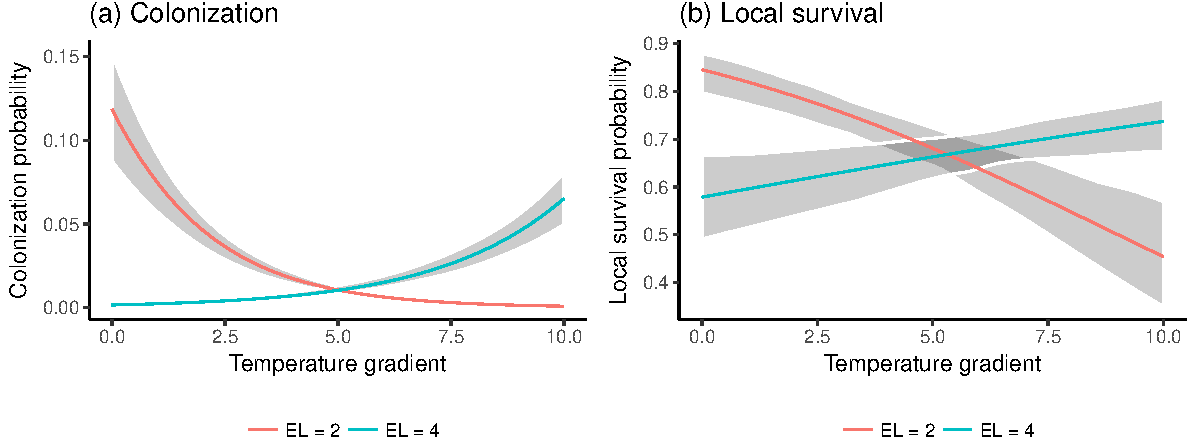
\includegraphics[width=1\linewidth]{Manuscript_files/figure-latex/Teff-1} \caption{Colonization (a) and local survival (b) of low temperature species (Ellenberg T = 2; red line) and high temperature species (Ellengerg T = 4) species along the temperature gradient. Given are means and 95\%-Credible Intervals from logistic linear mixed models.}\label{fig:Teff}
\end{figure}

\begin{figure}
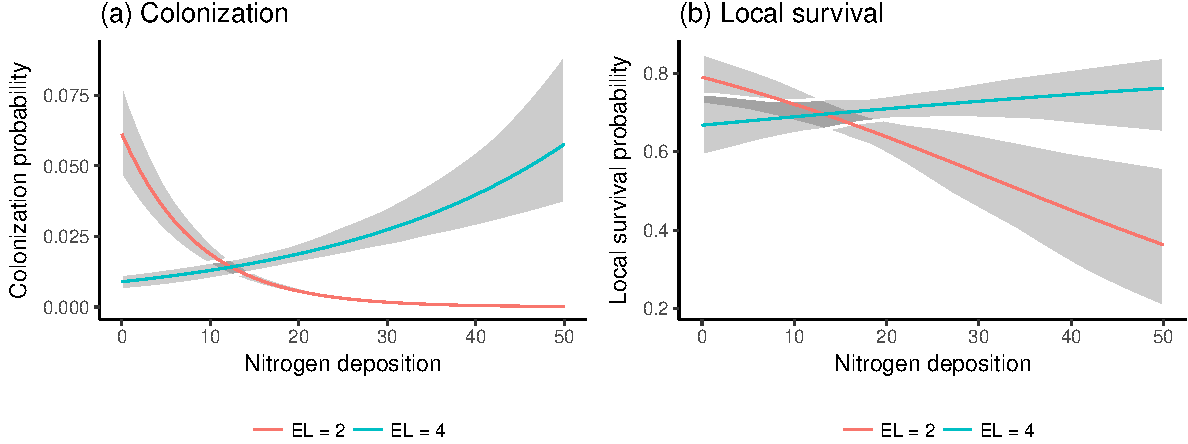
\includegraphics[width=1\linewidth]{Manuscript_files/figure-latex/Neff-1} \caption{Colonization (a) and local survival (b) of oligotrophic (Ellenberg N = 2; red line) and eutrophic (Ellengerg N = 4) species along the N deposition gradient. Given are means and 95\%-Credible Intervals from logistic linear mixed models.}\label{fig:Neff}
\end{figure}

For the temperature driven and nitrogen driven models in Table
\ref{tab:resdifeffects} we additionally tested whether the strength of
the effects on colonization probability and local survival differed from
the first/second to the second/third survey period. For the temperatur
driven models we found that the differences how species with different
Ellenberg T values responded to the average annual temperature of a site
tended to decrease from the first/second study period to the
second/third study period (colonization probability: period x Ellenberg
T x annual mean temperature of site = -0.0098, p = 0.70; local survival:
period x Ellenberg T x annual mean temperature of site = -0.072, p =
0.051). In contrast, however, the differences how species with different
Ellenberg N values responded to the average N deposition of a site
tended to increase from the first/second study period to the
second/third study period (colonization probability: period x Ellenberg
N x N deposition at site = 0.025, p = 0.74; local survival: period x
Ellenberg N x N deposition at site = 0.075, p = 0.50).

\begin{verbatim}
## Data: tt
## Models:
## m2: CI ~ Type + yr + (yr | aID_STAO)
## m1: CI ~ Type * yr + (yr | aID_STAO)
##    Df     AIC     BIC logLik deviance  Chisq Chi Df Pr(>Chisq)  
## m2  7 -246.90 -214.28 130.45  -260.90                           
## m1  8 -248.44 -211.16 132.22  -264.44 3.5419      1    0.05984 .
## ---
## Signif. codes:  0 '***' 0.001 '**' 0.01 '*' 0.05 '.' 0.1 ' ' 1
\end{verbatim}

\begin{verbatim}
## Generalized linear mixed model fit by maximum likelihood (Laplace
##   Approximation) [glmerMod]
##  Family: poisson  ( log )
## Formula: SR ~ yr * NTOT * Temperature + (1 | aID_STAO)
##    Data: surv
## 
##      AIC      BIC   logLik deviance df.resid 
##   2718.9   2754.6  -1350.5   2700.9      381 
## 
## Scaled residuals: 
##      Min       1Q   Median       3Q      Max 
## -2.51161 -0.38950 -0.00348  0.37725  2.19699 
## 
## Random effects:
##  Groups   Name        Variance Std.Dev.
##  aID_STAO (Intercept) 0.03294  0.1815  
## Number of obs: 390, groups:  aID_STAO, 130
## 
## Fixed effects:
##                       Estimate Std. Error z value Pr(>|z|)    
## (Intercept)          3.8808142  0.0268047 144.781   <2e-16 ***
## yr                   0.0029242  0.0027364   1.069   0.2852    
## NTOT                -0.0221202  0.0580005  -0.381   0.7029    
## Temperature         -0.0259552  0.0112875  -2.299   0.0215 *  
## yr:NTOT             -0.0079678  0.0059621  -1.336   0.1814    
## yr:Temperature       0.0002304  0.0011735   0.196   0.8444    
## NTOT:Temperature    -0.0148305  0.0154851  -0.958   0.3382    
## yr:NTOT:Temperature  0.0016841  0.0015971   1.054   0.2917    
## ---
## Signif. codes:  0 '***' 0.001 '**' 0.01 '*' 0.05 '.' 0.1 ' ' 1
## 
## Correlation of Fixed Effects:
##             (Intr) yr     NTOT   Tmprtr yr:NTOT yr:Tmp NTOT:T
## yr           0.019                                           
## NTOT        -0.612 -0.023                                    
## Temperature  0.249  0.014 -0.366                             
## yr:NTOT     -0.024 -0.626  0.044  0.005                      
## yr:Tempertr  0.014  0.310  0.005  0.030 -0.393               
## NTOT:Tmprtr  0.274 -0.002 -0.798 -0.063 -0.039  -0.045       
## yr:NTOT:Tmp  0.000  0.255 -0.040 -0.046 -0.776  -0.064  0.089
## convergence code: 0
## Model failed to converge with max|grad| = 0.00224997 (tol = 0.001, component 1)
## Model is nearly unidentifiable: very large eigenvalue
##  - Rescale variables?
\end{verbatim}

\begin{figure}
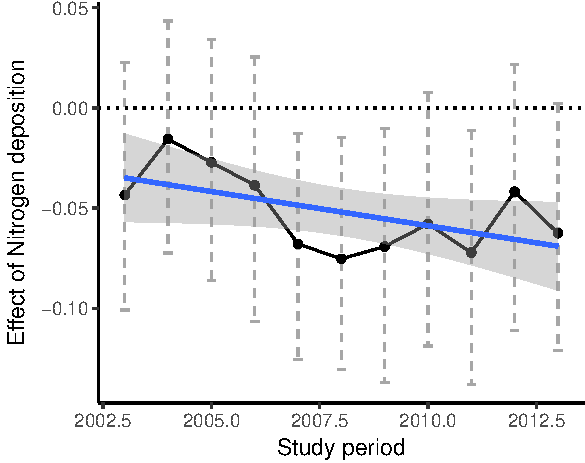
\includegraphics[width=1\linewidth]{Manuscript_files/figure-latex/figconsequences-1} \caption{Beschreibung einfügen.}\label{fig:figconsequences}
\end{figure}

It thus seems that temperature is the main driver of species turnover in
the first part of the study period and its importance is slightly
decreasing over time and nitrogen deposition becomes relatively more
important as a driver that shapes the species communities. We thus
expect to see that the correlation of the mean temperature value of a
community with the yearly annual temperature of the site (temperature
correlation) is decreasing over the years while the correlation of the
mean nutrient value of a community with the N deposition of the site
(nitrogen correlation) is increasing over the years. Our results tent to
be in line with this expectation (linear model: temporal trend of
temperature correlation x temporal trend of nitrogen correlation =
-0.0018, p = 0.16), however the change in the correlation over the study
period remained week and the temperature correlation remained stronger
than the nitrogen correlation over the entire study period (Left panel
of Fig. \ref{fig:figconsequences}). More important, however, was the
effect on our model that we used to infer whether and how strong the
spatial variation in N deposition is correlated with Nitrogen
deposition. If we apply that model the estimated effect of N depositon
on total species richness is increasing over the study period (right
panel of \ref{fig:figconsequences}).

\section*{Discussion}\label{discussion}
\addcontentsline{toc}{section}{Discussion}

\begin{itemize}
\tightlist
\item
  Any empty space that could be caused by any disturbance that let to
  the local disappearance of species is likely to be fiellied by
  eutrophic species. Disturbance depends on the site, while colonization
  depends on species characteristics.
\end{itemize}

-The rather large spatial turnover might be partly explained by species
that remained undetected in one of the surveys, but it might also be the
result of species that newly colonized sites (species gains) and species
that truely disappeared from sites (species losses).

\begin{itemize}
\item
  Altough N deposition considerabely declinded between 2005 and 2015, we
  could not detect major shifts in plant community structure during the
  same time period.
\item
  Eutrophic species have rather high local survival across the entire
  deposition gradient, while oligotrophic species have much reduced
  local survival at high N deposition. This suggests that it takes much
  more time to replace eutrophic by oligotrophic species than replacing
  oligotrophic by eutrophic species.
\item
  Our data on colonization and local survival (i.e.~temporal variation)
  confirm the empirical critical loads that we infered from anlysing
  spatial co-variation of N deposition and species richness.
\item
  Local survival is higher for low temperature plants --\textgreater{}
  This could explain the decrease in cumminity change along elevation.
  This could also explain the differences at mount summets were space
  was empty in the beginning.
\item
  Climatic effects are more likely to be reversed thant effects due to
  fertilization.
\end{itemize}

\subsubsection{Space for time
substitution}\label{space-for-time-substitution}

Often observational studies infer the change of plant diversity along a
gradient of N deposi- tion. Thus, they infer how the spatial variation
in species richness is related to N deposition and assume that this
spatial variation in species richness arose because over time some areas
lost more species than others because they chronically experienced
higher N deposition. Alt- hough there is evidence supporting the use of
such a `space for time substitution' for detecting the effects of N
deposition on plant diversity (Stevens et al. 2010), they can not
replace stud- ies that relate temporal patterns in species with N
deposition (De Schrijver et al. 2011). While recovery of acidified
surface waters has been well investigated (De Vries et al. 2015), there
are only a limited number of studies inferring temporal trends of plant
species diversity relat- ed to varying amounts of N-deposition. Storkey
et al. (2015) demonstrated a positive response of biodiversity to
reducing N addition from either atmospheric pollution or fertilizers in
the Park Grass Experiment: «The proportion of legumes, species richness
and diversity increased across the experiment between 1991 and 2012 as
N-deposition declined». For forest floor vegetation in permanent plots
across Europe the exceedance of critical loads of N over a peri- od from
9 to 42 years had negative effects on the cover of oligotrophic plant
species, i.e spe- cies that prefer nutrient-poor soils, although species
richness remained constant (Dirnböck et al. 2014). Another example of
recovery in eutrophicated habitats gives the recovery of species
richness in previously fertilized plots (Clark and Tilman 2008). In this
study, the recorded recovery in species richness within one or two
decade was likely due to the species rich vege- tation surrounding the
experimental plots, from where immigration was easily feasible.

\begin{quote}
Hier sagen, dass der CRL identisch wie der CRL von räumlichen
Zusammenhängen ist.
\end{quote}

\section*{Conclusions}\label{conclusions}
\addcontentsline{toc}{section}{Conclusions}

xxx

\section*{Acknowledgements}\label{acknowledgements}
\addcontentsline{toc}{section}{Acknowledgements}

We thank the dedicated and qualified botanists who conducted fieldwork.
The Swiss Federal Office for the Environment (FOEN) kindly provided
biodiversity monitoring data and topographic data. This work was
supported by the FOEN, the Swiss National Science Foundation (grant no.
31003A\_156294), the Swiss Association Pro Petite Camargue Alsacienne,
the Fondation de bienfaisance Jeanne Lovioz, and the MAVA Foundation.

\section*{References}\label{references}
\addcontentsline{toc}{section}{References}

\hypertarget{refs}{}
\hypertarget{ref-Hillebrand2018}{}
Hillebrand, Helmut, Bernd Blasius, Elizabeth T. Borer, Jonathan M.
Chase, John A. Downing, Britas Klemens Eriksson, Christopher T.
Filstrup, et al. 2018. ``Biodiversity Change Is Uncoupled from Species
Richness Trends: Consequences for Conservation and Monitoring.''
\emph{Journal of Applied Ecology} 55 (1): 169--84.
doi:\href{https://doi.org/10.1111/1365-2664.12959}{10.1111/1365-2664.12959}.



\end{document}
